\newpage
\section{Premiere impl\'ementation triviale d'un DHT}

L'impl\'ementation actuelle repose sur une architecture d\'ecentralis\'ee o\`u chaque unit\'e logicielle agit de mani\`ere autonome. Le syst\`eme \'evolue suivant une progression logique, partant de l'entit\'e de calcul jusqu'\`a la gestion fine de la circulation de l'information.

\subsection{L'Entit\'e de Base : Du N\oe ud au Thread}
Le choix fondamental de conception est de repr\'esenter chaque n\oe ud par un \texttt{NodeThread}. Dans ce mod\`ele, le multi-threading simule l'isolation des machines d'un r\'eseau distribu\'e. Comme l'illustre la Figure~\ref{fig:node_thread_architecture}, chaque n\oe ud poss\`ede son propre cycle de vie (\texttt{run()}) et ses ressources internes.

\begin{figure}[H]
    \centering
    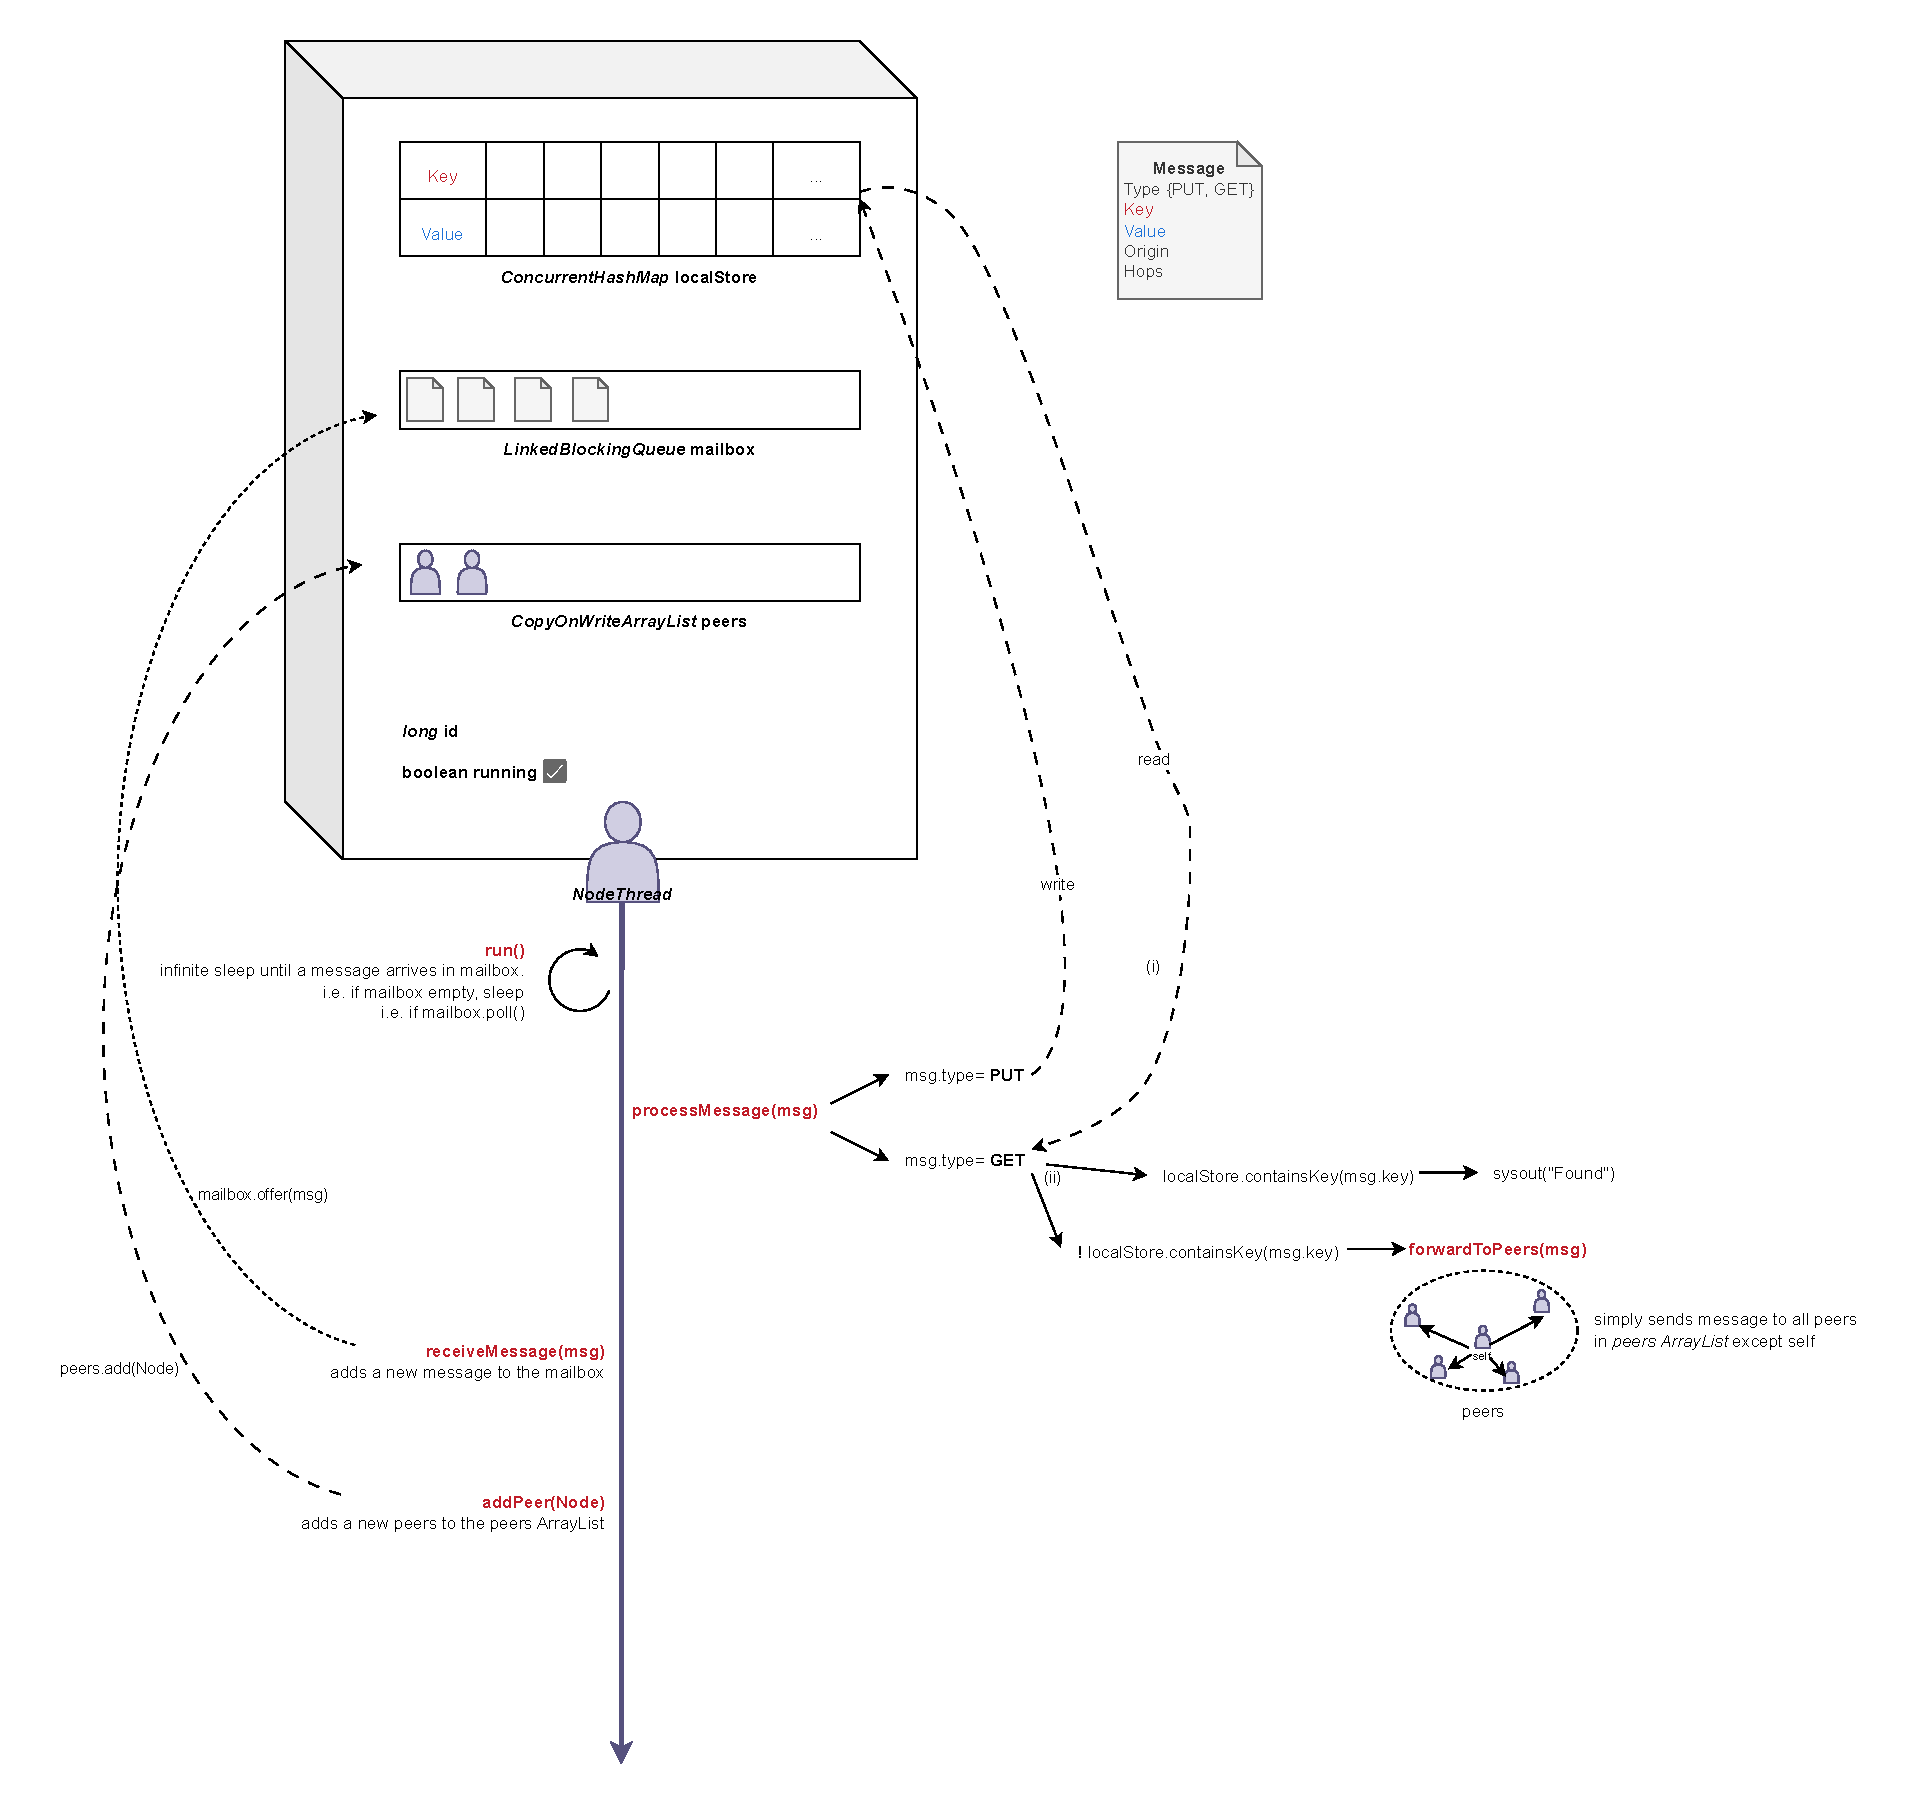
\includegraphics[width=0.8\textwidth]{figures/NodeThread.drawio.pdf}
    \caption{\textbf{Architecture interne et fonctionnement du \texttt{NodeThread}.} Ce diagramme d\'etaille la composition d'un n\oe ud. La fl\`eche verticale symbolise le thread actif, tandis que la bo\^ite 3D repr\'esente l'objet \texttt{Node} avec son \'etat (\texttt{id}, \texttt{running}) et ses structures (\texttt{peers}, \texttt{localStore}). La structure \texttt{Message} est dessin\'ee en gris pour montrer qu'elle est stock\'ee dans la \texttt{mailbox}. Les mots cl\'es Key et Value sont mis en \'evidence pour montrer le transfert d'information du message vers le stockage local. Les fonctions principales sont aussi d\'ecrites : \texttt{run()} maintient le n\oe ud actif, \texttt{receiveMessage()} ajoute les requ\^etes \`a la file, et \texttt{processMessage()} traite la logique m\'etier.}
    \label{fig:node_thread_architecture}
\end{figure}

Pour garantir la stabilit\'e de ce mod\`ele face aux acc\`es concurrents, nous choisissons des structures de donn\'ees sp\'ecifiques :
\begin{itemize}
    \item \textbf{Le Stockage (\texttt{localStore})} : L'utilisation d'une \texttt{ConcurrentHashMap} est indispensable. Elle permet \`a un thread de lire une donn\'ee (\texttt{GET}) pendant qu'un autre message de type \texttt{PUT} met \`a jour la table, \'evitant ainsi les corruptions de donn\'ees.
    \item \textbf{La Liste de Voisinage (\texttt{peers})} : Impl\'ement\'ee via une \texttt{CopyOnWriteArrayList}, elle permet de parcourir les voisins en toute s\'ecurit\'e. Cette structure est optimale car les voisins changent peu apr\`es la phase de d\'ecouverte, mais sont consult\'es \`a chaque transfert de message.
\end{itemize}

\subsection{Le M\'ecanisme de Communication : La Mailbox}
Une fois les n\oe uds actifs, ils communiquent via une \texttt{mailbox} impl\'ement\'ee par une \texttt{LinkedBlockingQueue}. Ce m\'ecanisme permet de d\'ecoupler l'envoi de la r\'eception. Le choix de la m\'ethode d'insertion est ici strat\'egique :
\begin{itemize}
    \item \textbf{L'avantage de \texttt{offer()}} : Contrairement \`a \texttt{add()} ou \texttt{put()}, la fonction \texttt{receiveMessage(msg)} utilise \texttt{mailbox.offer(msg)}. C'est une tentative non-bloquante qui ajoute le message \`a la file sans interrompre l'exp\'editeur. Cela pr\'evient les \textit{deadlocks} (blocages mutuels) o\`u deux n\oe uds s'attendraient ind\'efiniment.
\end{itemize}

\subsection{\'Evolution du Message : Du simple "Sender" \`a l'"Origin"}
La gestion des messages constitue le c\oe ur du routage. L'analyse a montr\'e qu'en relayant un message, le n\oe ud receveur perdait la trace de l'initiateur, rendant la r\'eponse impossible.

Comme l'illustre la Figure \ref{fig:message_evolution}, nous sommes pass\'es d'une structure simple \`a une structure permettant le suivi :

\begin{figure}[H]
    \centering % This centers the group of two images on the page
    
    % --- Image 1: Message v0 (Reduced size) ---
    \begin{subfigure}[b]{0.2\textwidth} 
        \centering
        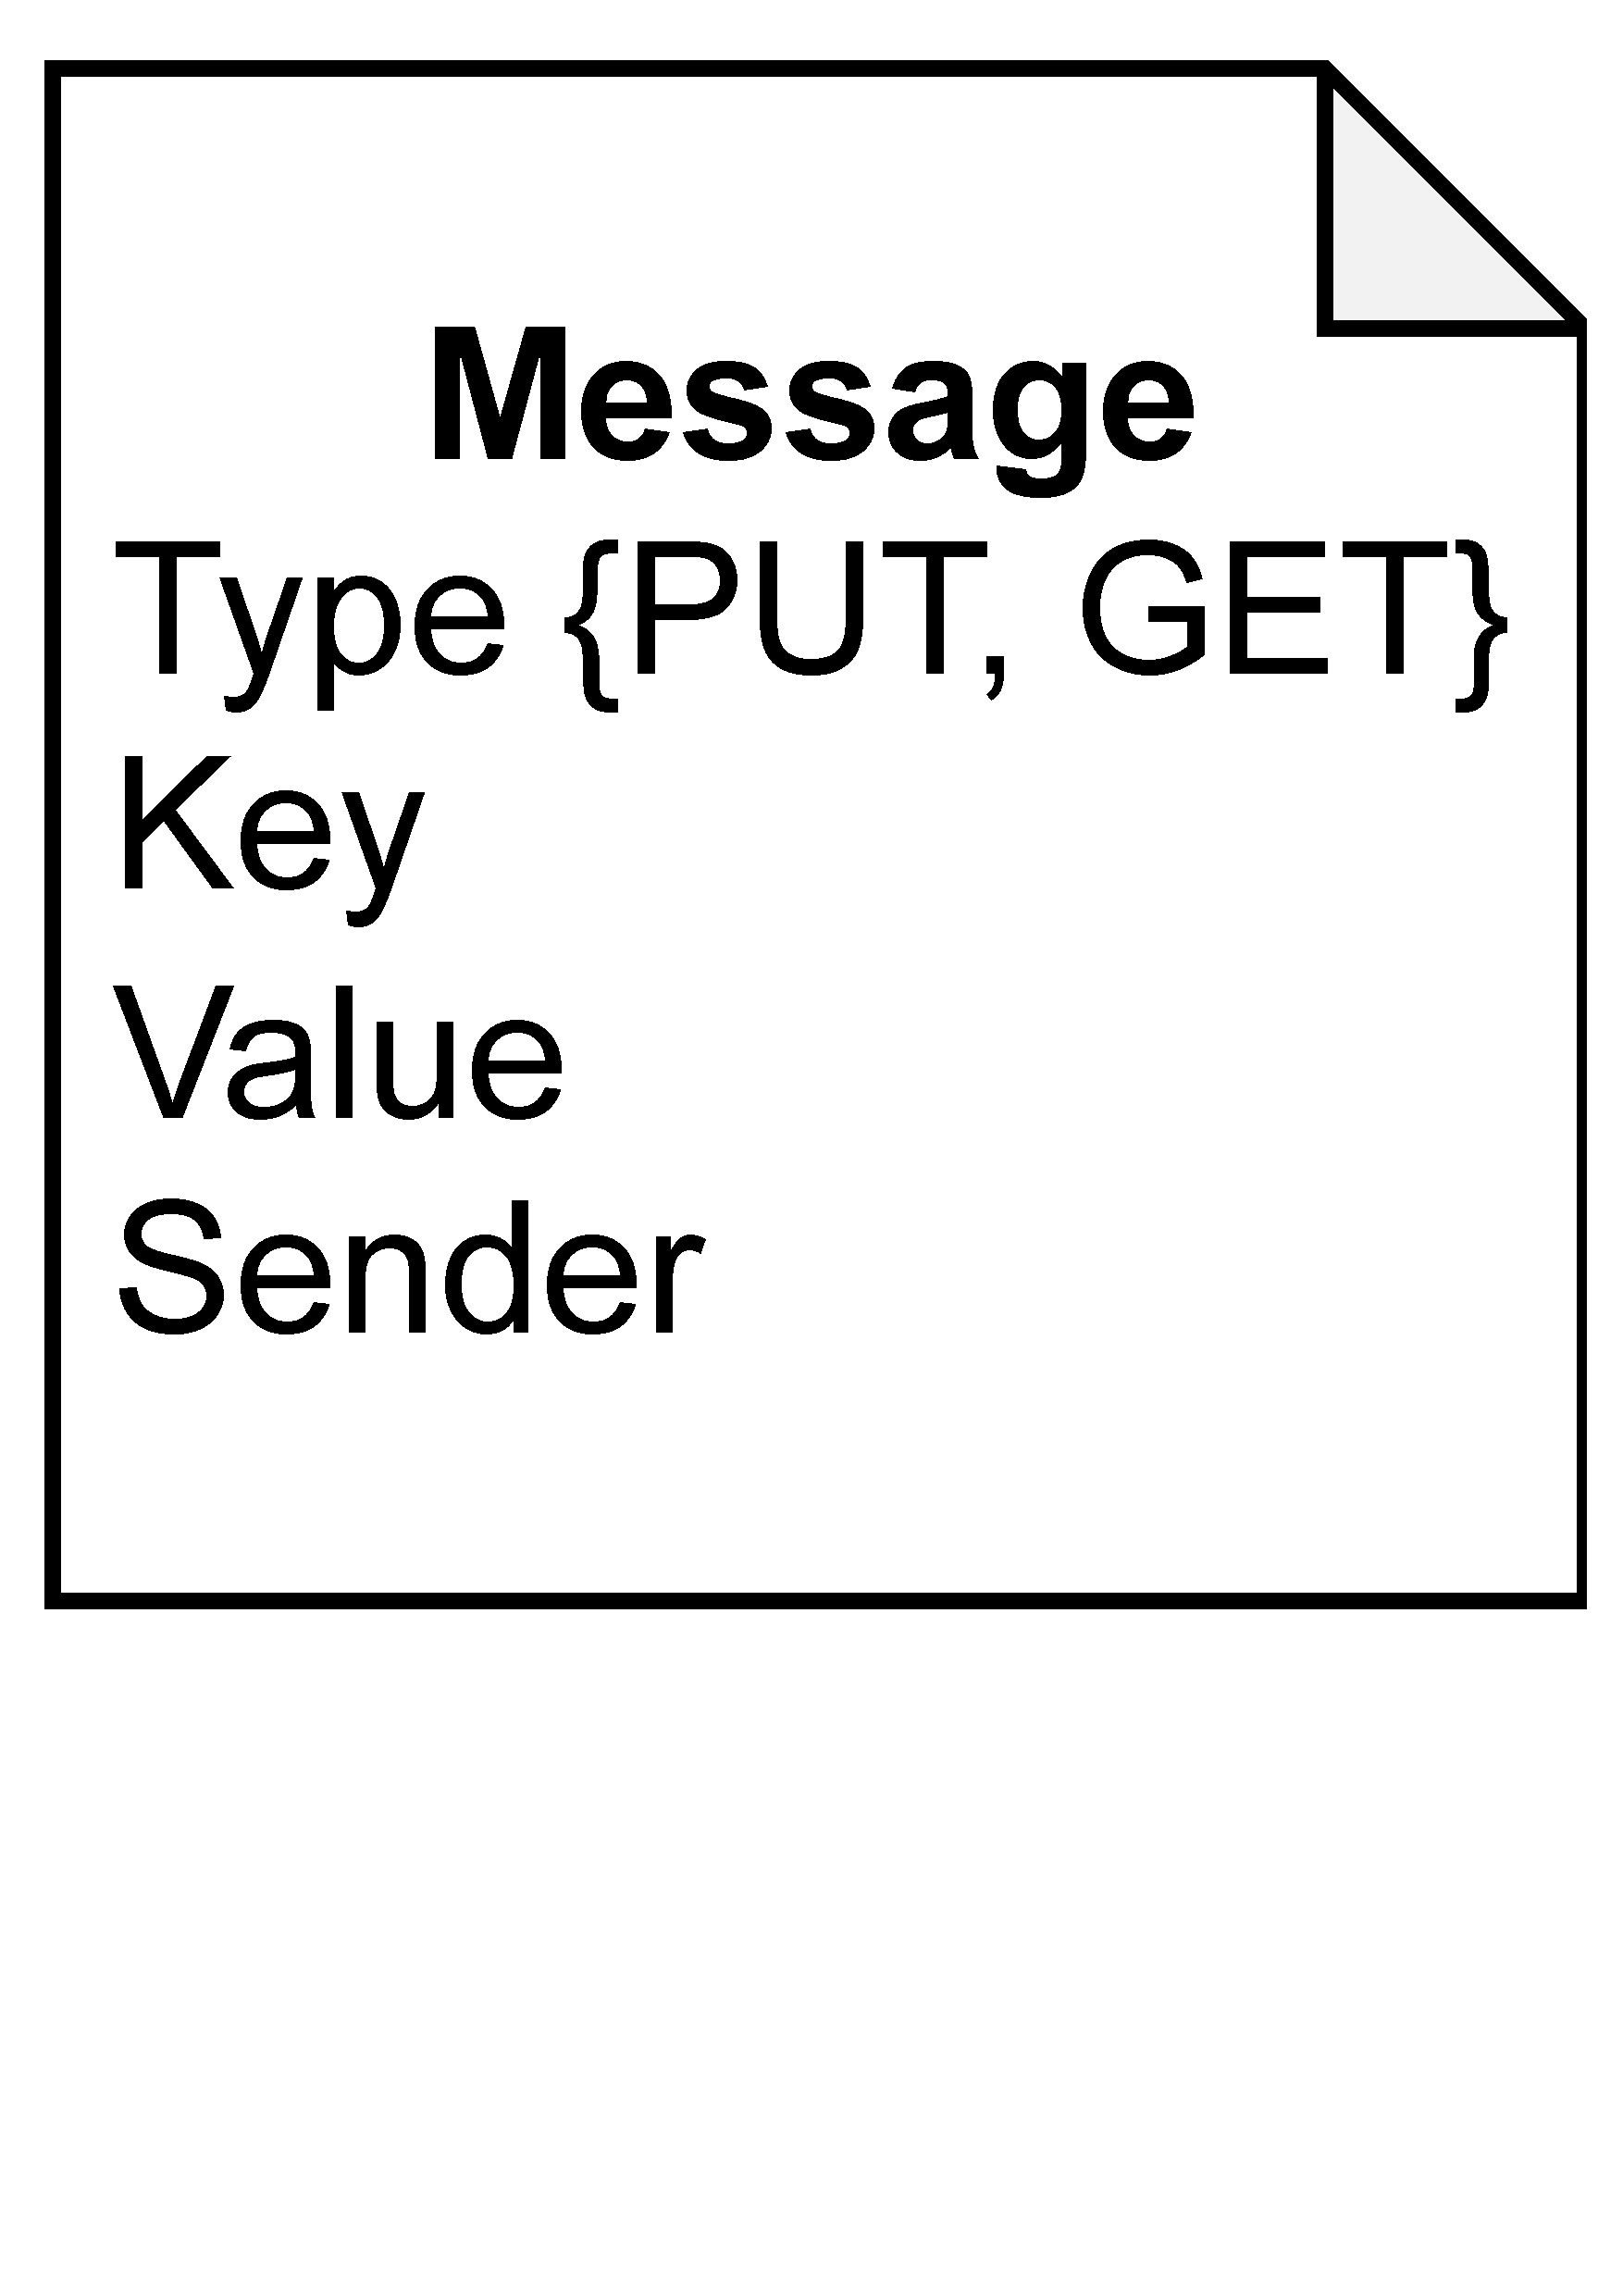
\includegraphics[width=\textwidth]{figures/Messagev0.drawio.pdf}
        \caption{\textbf{v0} : Limit\'e au \texttt{Sender}.}
        \label{fig:msg_v0}
    \end{subfigure}
    %
    \hspace{1cm} % Fixed space between images (keeps them close)
    %
    % --- Image 2: Message v1 (Reduced size) ---
    \begin{subfigure}[b]{0.2\textwidth} 
        \centering
        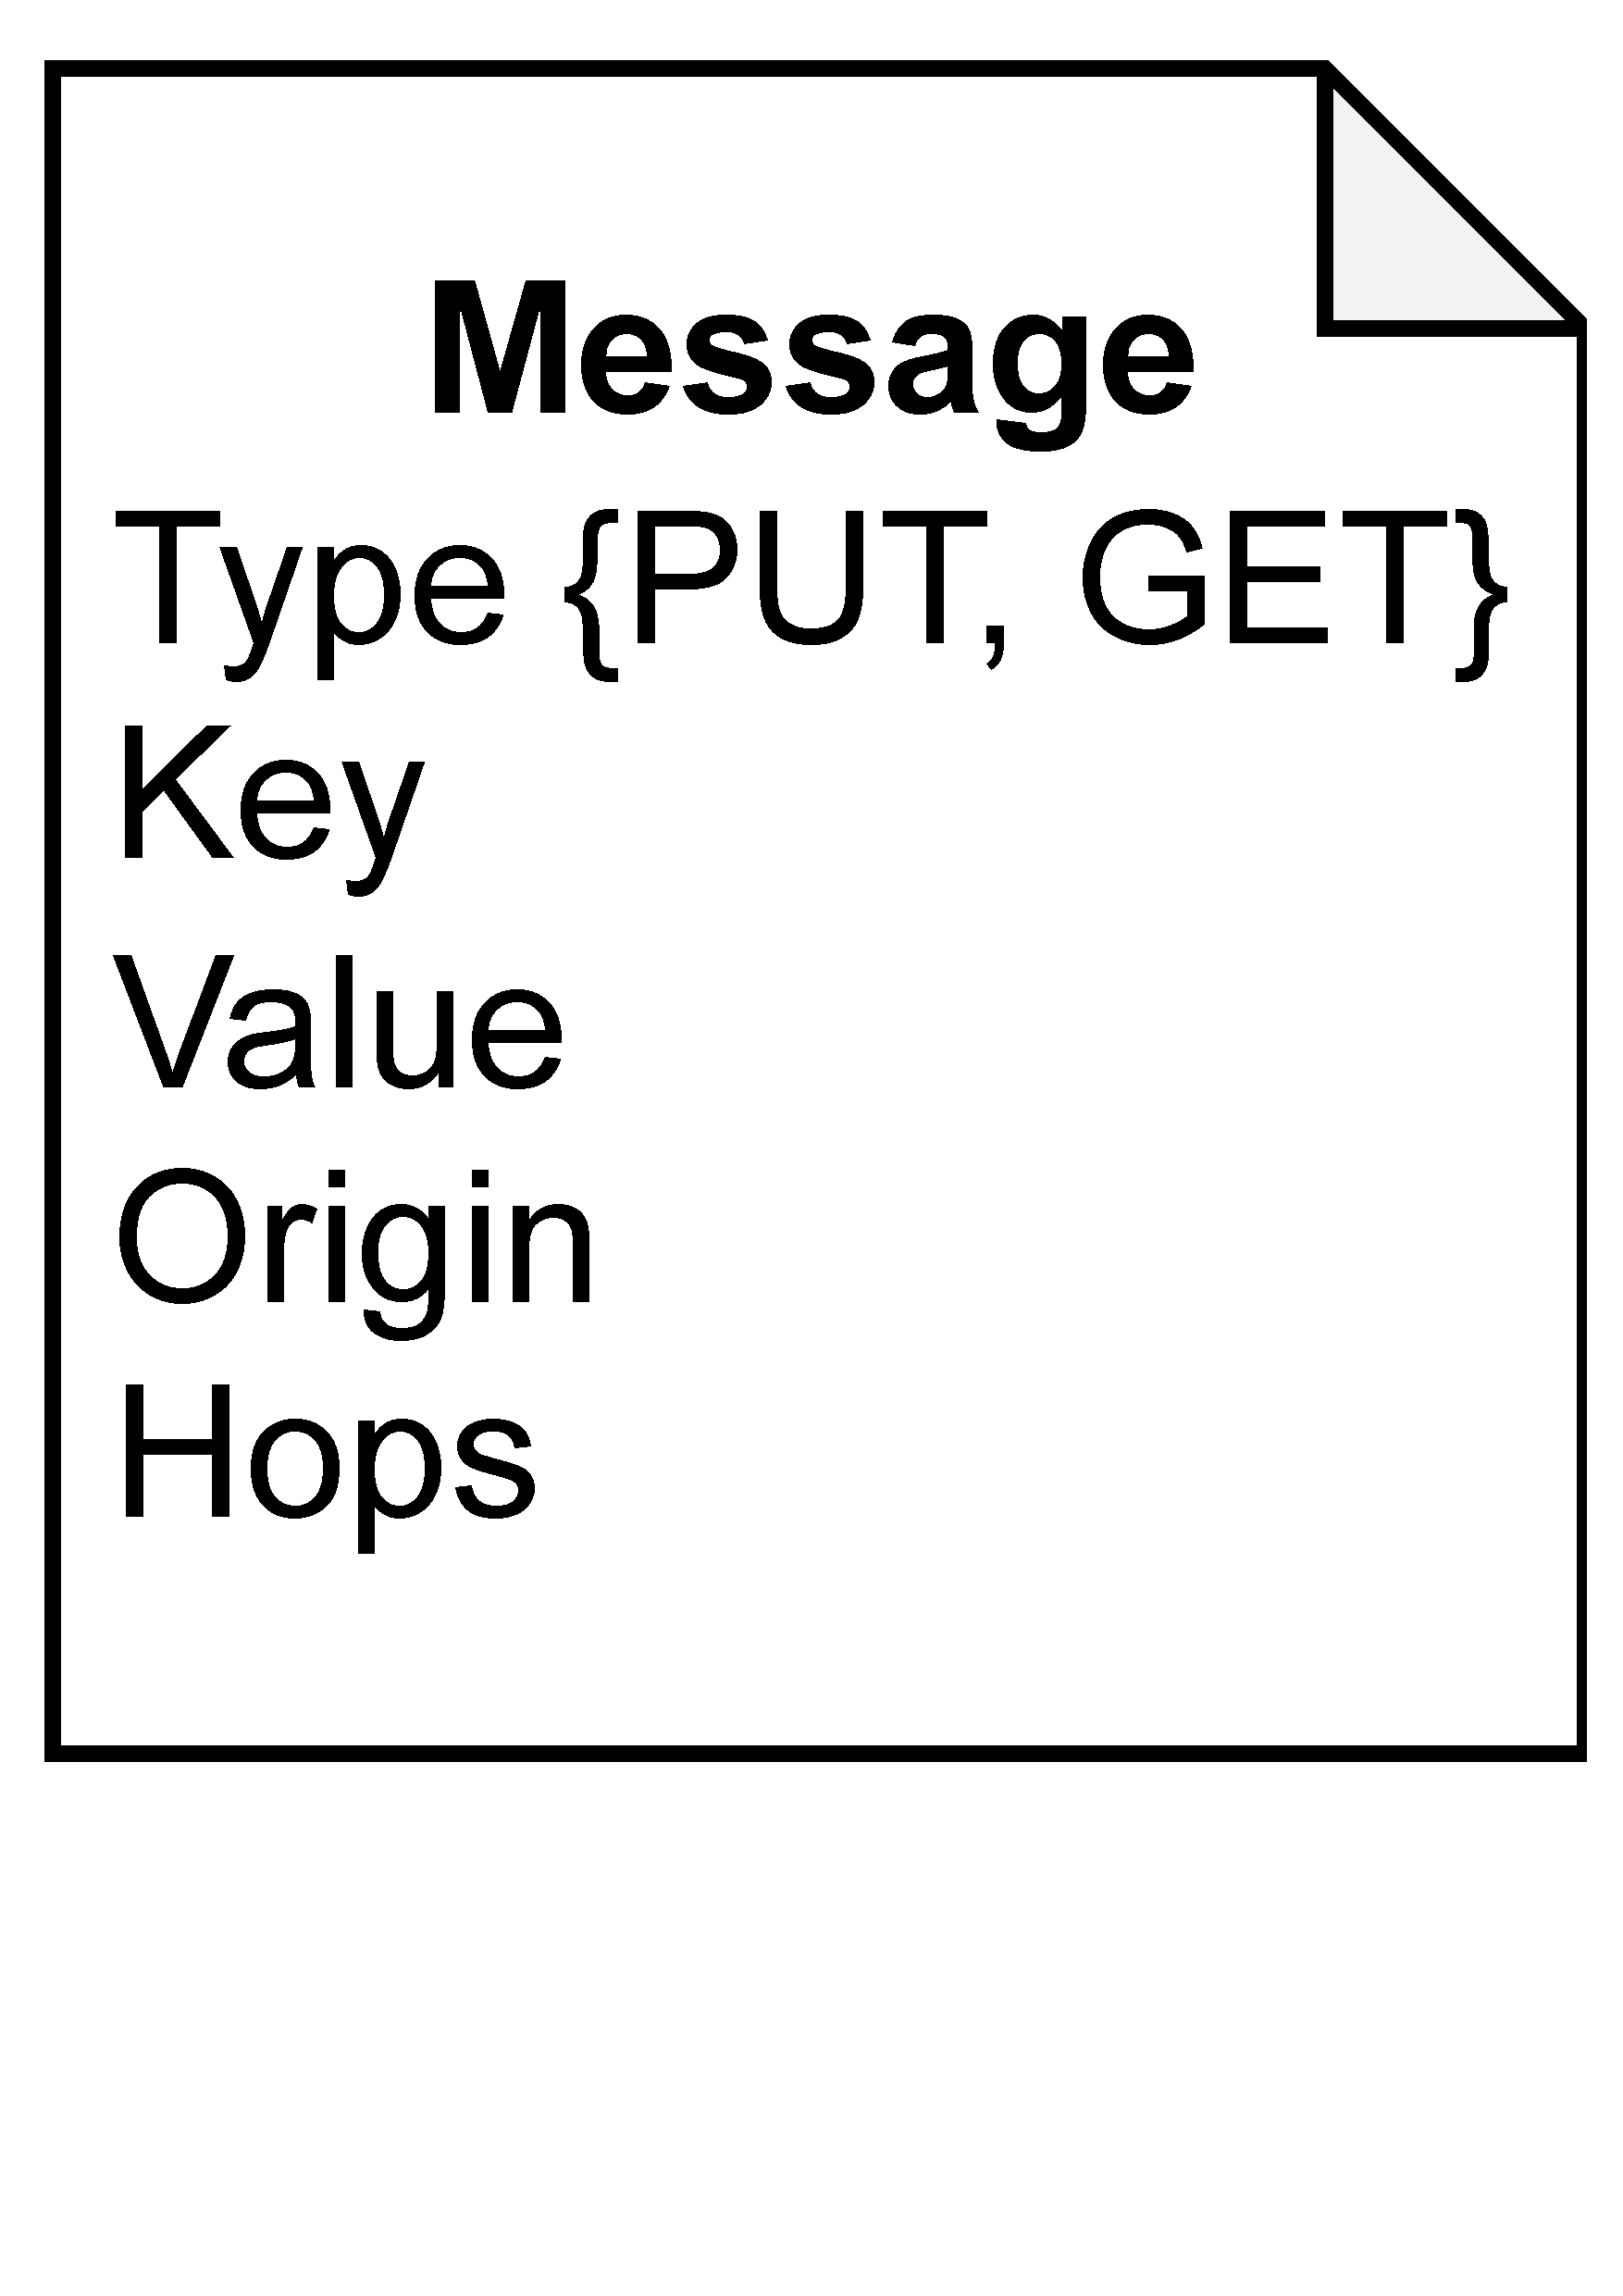
\includegraphics[width=\textwidth]{figures/Messagev1.drawio.pdf}
        \caption{\textbf{v1} : Ajout de \texttt{Origin}.}
        \label{fig:msg_v1}
    \end{subfigure}
    
    \caption{Comparaison de l'\'evolution de la structure du Message.}
    \label{fig:message_evolution}
\end{figure}

Dans la version initiale (\textbf{v0}), le message ne contenait que l'exp\'editeur imm\'ediat. La version actuelle (\textbf{v1}) remplace ce champ par l'\texttt{Origin}. En conservant cette r\'ef\'erence fixe, le message garde son identit\'e tout au long de son parcours.

\subsection{Mesure du parcours et topologie du syst\`eme}
Le \texttt{DHTSystem} orchestre le r\'eseau via deux \'etapes cl\'es : l'ajout de n\oe uds (\texttt{addNode}) et la cr\'eation de liens bidirectionnels (\texttt{buildDiscoveryChain}). Comme le montre la Figure~\ref{fig:dht_system_topology}, cette cha\^ine permet la propagation des messages de proche en proche. Pour diagnostiquer l'efficacit\'e de ce routage, nous int\'egrons un compteur de \texttt{Hops}. \`A chaque transfert vers un pair, ce compteur s'incr\'emente, permettant de d\'etecter les inefficacit\'es ou les recherches trop longues.

\begin{figure}[H]
    \centering
    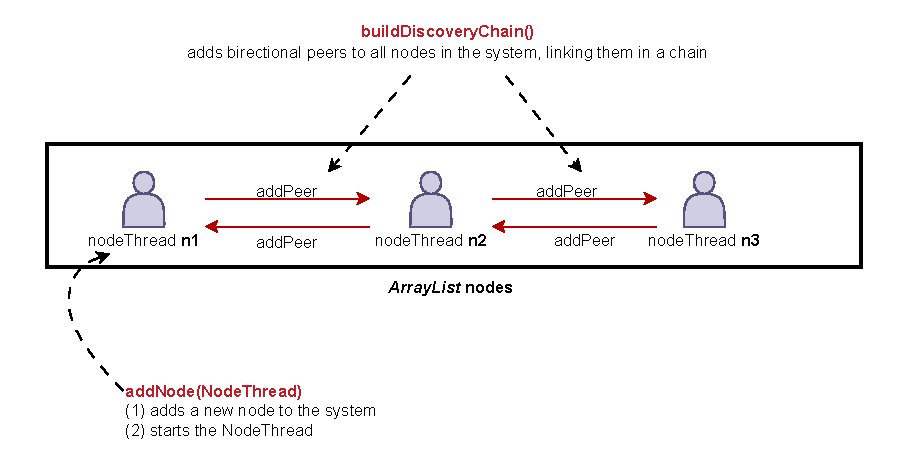
\includegraphics[width=0.8\textwidth]{figures/DHTSystem.drawio.pdf}
    \caption{\textbf{Topologie et initialisation du r\'eseau via \texttt{DHTSystem}.} Ce sch\'ema illustre l'organisation des n\oe uds stock\'es dans une \texttt{ArrayList}. En bas, la fonction \texttt{addNode()} est indiqu\'ee comme responsable de l'ajout d'un nouveau n\oe ud et du d\'emarrage de son thread. En haut, la fonction \texttt{buildDiscoveryChain()} est mise en \'evidence : elle parcourt la liste pour \'etablir des connexions bidirectionnelles entre les n\oe uds voisins. Ces connexions sont mat\'erialis\'ees par les fl\`eches rouges \texttt{addPeer}, transformant la simple liste en une cha\^ine de propagation op\'erationnelle.}
    \label{fig:dht_system_topology}
\end{figure}

\subsection{Analyse des Erreurs et Limites de la V0}

Cette premi\`ere impl\'ementation, bien que fonctionnelle pour les sc\'enarios nominaux, pr\'esente des failles critiques identifi\'ees lors des tests.

\subsection{Erreurs majeures rencontr\'ees}
\begin{itemize}
    \item \textbf{Boucles de recherche infinies} : Si une cl\'e demand\'ee n'existe pas dans le syst\`eme (ex: recherche de "Shape"), le message est transf\'er\'e de n\oe ud en n\oe ud sans jamais s'arr\^eter. Les threads continuent de saturer la file d'attente de leurs voisins ind\'efiniment.
    \item \textbf{Probl\`eme de Flooding} : Actuellement, un n\oe ud propage le message \`a \textit{tous} ses pairs. Dans un r\'eseau plus large, cela provoquerait une explosion exponentielle du nombre de messages, paralysant rapidement les ressources CPU et m\'emoire.
    \item \textbf{Absence de m\'ecanisme de retour} : Lorsqu'un n\oe ud trouve une donn\'ee, il se contente d'afficher "FOUND" dans la console. L'origine de la requ\^ete n'est jamais notifi\'ee formellement par le biais d'un message retour.
\end{itemize}

\subsection{Points d'am\'eliorations pour la V1}
Pour stabiliser le syst\`eme, les \'evolutions suivantes sont prioritaires :
\begin{enumerate}
    \item \textbf{Time To Live (TTL)} : Int\'egrer une limite de sauts au sein de la classe \texttt{Message}. Une fois le compteur \`a z\'ero, le message est supprim\'e, stoppant ainsi les recherches infructueuses.
    \item \textbf{Type RESPONSE} : Cr\'eer un nouveau type de message pour permettre l'acheminement de la valeur trouv\'ee directement vers l'initiateur (\texttt{Origin}).
    \item \textbf{M\'emorisation des requ\^etes} : Faire en sorte que chaque n\oe ud garde en m\'emoire les identifiants des messages d\'ej\`a trait\'es pour \'eviter de relayer plusieurs fois la m\^eme requ\^ete.
\end{enumerate}